
\section{Teknologibeskrivelse} \label{sec:teknologibeskrivelse}
Aktivitetsarmbånd bliver i stigende grad mere udbredt. Ifølge International Data Corporation er der sket en stigning i salget af aktivitetsarmbånd fra $11,8$ millioner enheder i første kvartal af 2015 til $19,7$ millioner i første kvartal af 2016 \citep{IDC2016}.

Det er fundet, at Fitbit udgør en stor andel af markedet for aktivitetsarmbånd og, at der fra første kvartal i 2015 til første kvartal i 2016, er sket en stigning i salget på $1$ million enheder \citep{IDC2016}.  
Fitbit Flex ses på \autoref{fig:fitbitflexarmbånd}. 

\begin{figure}[H]
	\centering
	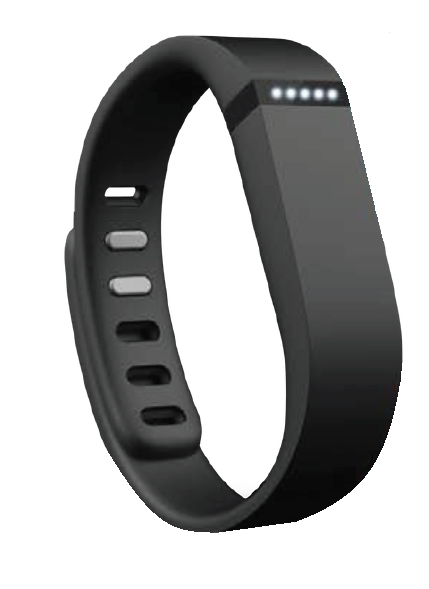
\includegraphics[width=0.3\textwidth]{figures/fitbitflex}
	\caption{Fitbit Flex armbånd \citep{fitbitflex}.}
	\label{fig:fitbitflexarmbånd}
\end{figure}

\noindent
Overordnet består Fitbit Flex med tilbehør af en flex tracker, oplader kabel, trådløs synkroniserings dongle og armbånd til flex tracker \citep{fitbitflex}. Disse kan ligeledes ses af \autoref{fig:fitbitflexindhold}. 

\begin{figure}[H]
	\centering
	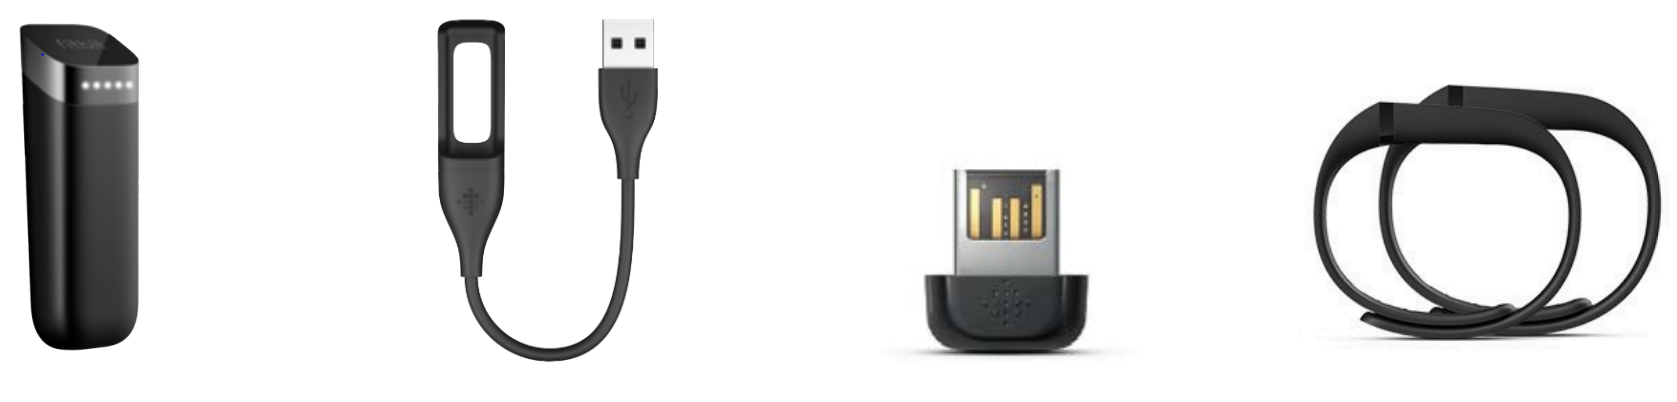
\includegraphics[width=0.6\textwidth]{figures/fitbitflexindhold}
	\caption{Fra venstre mod højre ses de forskellige dele af Fitbit Flex pakken, bestående af flex tracker, oplader kabel, trådløs synkroniserings dongle og armbånd \citep{fitbitflex}.}
	\label{fig:fitbitflexindhold}
\end{figure}

\noindent
Fitbit Flex er i stand til at måle antal minutter, brugeren er aktiv, længden samt kvalitet af søvn og antal skridt, hvorudfra den kan estimere forbrændte kalorier og afstand dækket. 
For at brugeren kan se den registrerede aktivitet, som er blevet opsamlet af armbåndet, skal dette synkroniseres med en kompatibel enhed, da armbåndet kun besidder et display bestående af fem LED'er \citep{fitbitflex}. 

Synkronisering foregår trådløst ved brug af bluetooth low energy (BLE) og kan foregå mellem forskellige enheder såsom smartphone og computer. 
Synkronisering mellem flex tracker og computer kræver dog anvendelse af den trådløse synkroniserings dongle, der ses af \autoref{fig:fitbitflexindhold}.
Forudsætninger for, at data kan synkroniseres er, at en kompatibel enhed har den korrekte applikation installeret, hvor synkroniseringen ellers sker automatisk idet applikationen åbnes.  
Yderligere skal der oprettes en brugerkonto på \url{www.fitbit.com}, hvor brugeren oplyser personlige informationer: køn, alder, højde og vægt. Dette er nødvendigt i forhold til optimering af dataopsamling og estimering af forbrændte kalorier \citep{fitbitflex}.  

Gennem applikationen visualiseres den registrerede aktivitet, hvor brugeren har mulighed for at se data fra anvendelsesperioden. Data kan også observeres på Fitbits hjemmeside, hvor det er muligt at logge ind via brugerkontoen. 
Således ville alle i besiddelse af en given brugerkonto have adgang til den synkroniserede data, uden fysisk at have hverken bruger eller armbånd til stede. 
Til den daglige aktivitet har brugeren mulighed for at sætte bestemte mål til den fysiske aktivitet. Alt efter hvilke mål brugeren sætter for sig selv, kan progressionen ses ud fra de fem LED'er på armbåndet ved, at brugeren trykker to gange på armbåndet \citep{fitbitflex}.   

Når ét af brugerens mål gennemføres, visualiseres dette ved, at de 5 LED'er blinker, og at armbåndet vibrerer. 
Fitbit Flex er ikke i stand til at visualisere batteriniveauet for armbåndet, dette kan dog ses ved brug af applikationen. 
Hukommelsen i flex trackeren tillader detaljeret data at blive lagret i perioder op til 7 dage og består af minut til minut målinger.  
Yderligere lagres summeringer af daglig aktivitet i op til 30 dage. 
Ved jævnlig synkronisering er det muligt for brugeren at bevare detaljeret data, da informationen tilknyttes brugerkontoen. 
Fitbit anbefaler én daglig synkronisering, dog er det ikke en nødvendighed \citep{fitbitflex}. 

\subsection{Hardware}
Fitbit Flex trackeren har forskellige hardware elementer, hvorfra trackeren signalerer, og detekterer fysisk aktivitet. Hardwaren i trackeren udgøres af et display, batteri, en sensor og motorer \citep{fitbitflex}.
 
\subsubsection{Display} 
Flex trackeren er udstyret med fem LED'er, der ved forskellige operationstilstande, såsom alarm, aktivitet eller søvntracking, signalerer til brugeren. 
LED'erne kan fungere som indikator for progressionen i forhold til det brugerdefinerede fysiske mål for dagen. Hertil vil hver LED repræsentere en procentvis progression i intervaller af $20~\%$. Ved $73~\%$ progression af det fysisk mål, vil de første tre LED'er lyse, og den fjerde vil blinke. Dette indikerer, at brugeren har nået $60~\%$ af målet, og at brugeren nu befinder sig mellem $60~\%$ og $80~\%$. 
Det samme gør sig gældende, når flex trackeren sættes til opladning. Her indikerer LED'erne, hvor langt armbåndet er fra fuld opladning, som signaleres ved, at alle fem LED'er lyser \citep{fitbitflex}. 
%I tilfælde af synkroniseringsfejl vil dette også fremgå af LED'erne. Her vil armbåndet lyse med et mønster, skiftevis mellem at have ingen eller alle LED'er tændt. 
%Ved manuel aktivering og de-aktivering af sleep mode, vil LED'erne indikere dette gennem forskellige indikationsmønstre.

\subsubsection{Sensor} 
Flex trackeren registrerer den fysiske aktivitet ved anvendelse af et 3 akses Mikro elektro-mekanisk accelerometer, hvilket er den eneste sensor, som er implementeret i armbåndet. Et 3-akses accelerometer kan måle i x-, y- og z-retning, og kan give et udtryk for ændringerne i hastigheden \citep{ravi2005}. Ud fra algoritmer analyseres bevægelsesmønstre, hvorved der kan oplyses hvor mange skridt der er foretaget under løb eller gang, den tilbagelagte afstand, med mere. 

\subsubsection{Motor}
Flex trackeren er udstyret med en vibrationsmotor, der aktiveres under forskellige funktioner, når armbåndet anvendes. Disse fungerer i sammenspil med displayet som et kommunikationsredskab for brugeren. Vibration aktiveres ved anvendelse af alarm funktion og ved aktivering eller deaktivering af sleep mode, samt når det daglige fysiske mål nåes. 

\subsubsection{Batteri} 
Fitbit Flex indeholder et genopladeligt batteri, der oplades ved brug af det medfølgende kabel. Dette ses af \autoref{fig:fitbitflexindhold}. Kablet tilsluttes en computer og opladningen begynder, hvis computeren er tændt. 
Levetiden på batteriet er op til 5 dage afhængigt af, hvor ofte armbåndet synkroniseres for at visualisere progressionen.


\subsection{Software}
Applikationen, som kan installeres på smartphone, er brugerfladen hvorfra den synkroniserede data formidles til brugeren. Her oplyses skridt, forbrændte kalorier med mere. 
Alt efter brugerens interesser, kan der også udfyldes informationer omkring indtaget kost ved brug af applikationen. Brugeren kan ud fra dette få et estimat af, hvor mange kalorier, der indtages, hvortil dette kan sammenlignes med antal kalorier forbrændt. Anvendelsen af denne funktion er dog ikke en nødvendighed for anvendelsen af Fitbit Flex eller applikationen, dog kunne dette give en praktiserende læge indblik i, om patienten overholder anbefalingerne for hypertensive patienter, både i forhold til kostvaner og fysisk aktivitet. 

\begin{figure}[H]
	\centering
	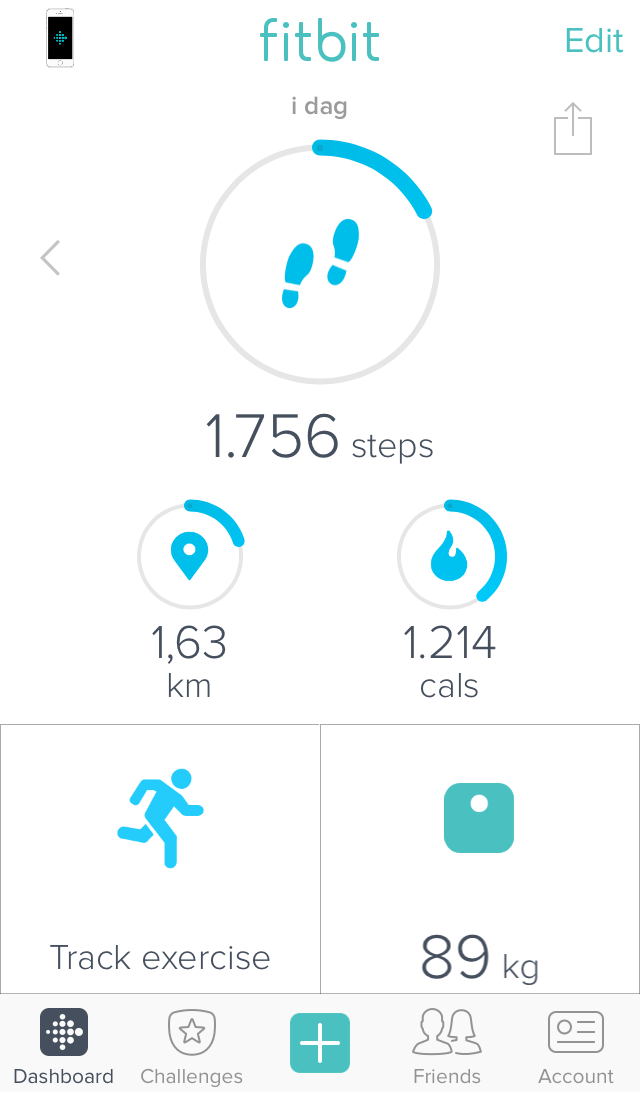
\includegraphics[width=0.45\textwidth]{figures/burgerfladeoversigt}
	\caption{Oversigt over fysisk aktivitet, der vises idet applikationen åbnes. Her ses blandt andet antal skridt taget, afstand dækket og kalorier forbrændt.}
	\label{fig:brugerfladeoversigt}
\end{figure}

\noindent
Af \autoref{fig:brugerfladeoversigt} ses oversigt over den registrerede aktivitet, som er målt gennem armbåndet. Her ses antal skridt taget, afstand dækket og kalorier forbrændt. Af oversigten ses også, hvor langt brugeren er fra at opfylde de forskellige aktivitetsmål og er repræsenteret af den blå cirkel omkring de forskellige angivelser. 
I bunden ses fire forskellige oversigter, hvor der fra venstre mod højre ses 'Dashboard', 'Challenges', 'Friends' og 'Account'. Plus-tegnet i midten fungerer som en genvej til forskellige funktioner under de fire oversigter. 
'Dashboard' er den overordnede oversigt, som oplyser det førnævnte.
'Challenges' viser en oversigt over tilvalgte aktivitetsudfordringer, hvor brugeren har mulighed for at opstille udfordringer med venner samt andre brugere af applikationen. 
'Friends' giver brugeren et overblik over venner, der er tilføjet til applikationen. 
'Account' viser et overblik over, hvilken bruger, der er logget ind, og hvilken Fitbit enhed, der er tilsluttet applikationen. Yderligere kan der foretages ændringer af profil og mål for daglig fysisk aktivitet. 

En detaljeret oversigt over ydet aktivitet kan ses under den overordnede oversigt ved at trykke på de specifikke målinger. Ved at trykke på 'Steps' ses eksemplet, der fremgår af \autoref{fig:brugerfladesteps}.  

\begin{comment} % Kan ikke henvise til disse figurer.
\begin{figure}[H]
	\centering
	\begin{minipage}[t]{0.45\textwidth}
		\label{fig:brugerfladesteps}
	    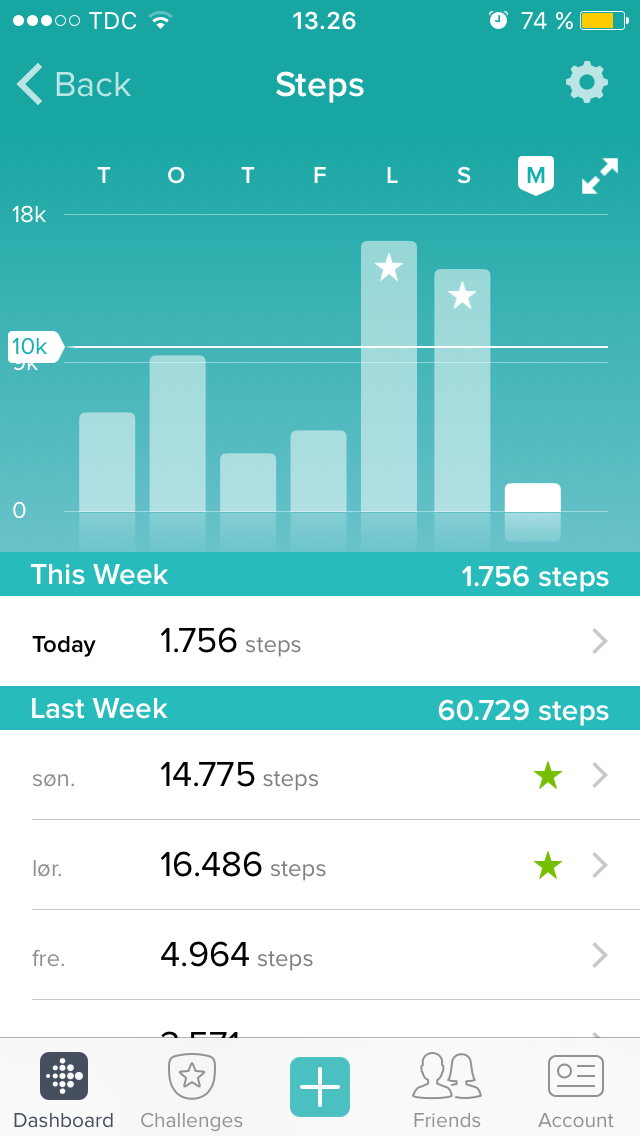
\includegraphics[width=0.45\textwidth]{figures/brugerfladesteps}
		\flushleft
		\textit{Oversigt over skridt taget for forhenværende dage, som graf (øverst) og tabel (nederst).}
	\end{minipage}
	\hfill
	\begin{minipage}[t]{0.45\textwidth}
		\label{fig:specifiksteps}
		\centering
		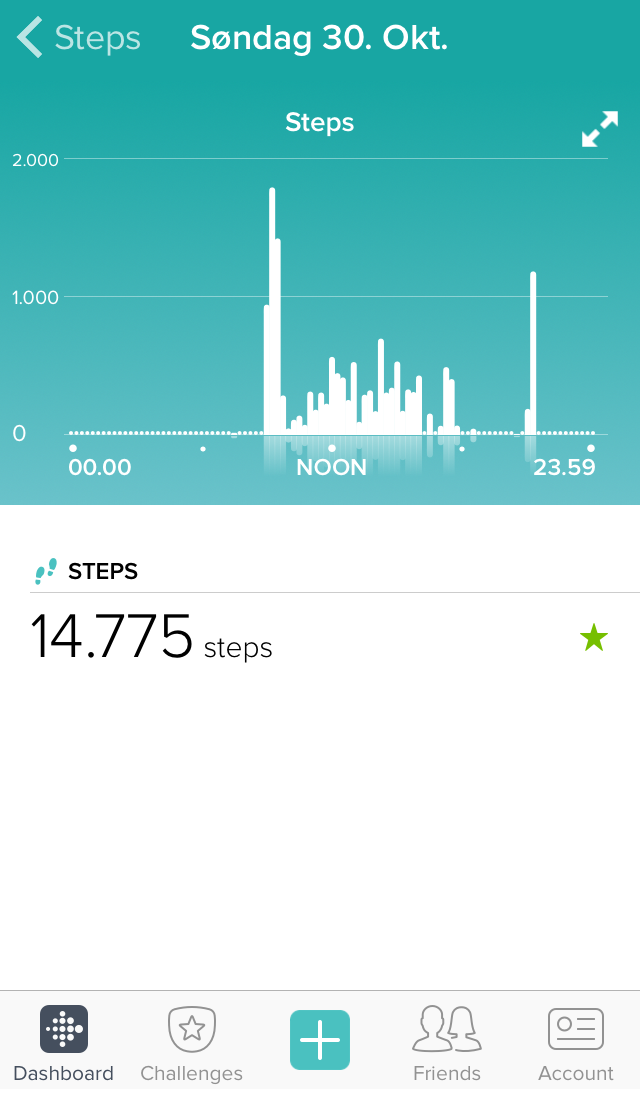
\includegraphics[width=0.45\textwidth]{figures/specifiksteps}
		\flushleft
		\vspace{12pt}
		\textit{Til venstre ses den grafiske oversigt over antal skridt taget, og højre figur viser skridt taget i en tabel.}
	\end{minipage}
\end{figure}
\end{comment}

\begin{figure}[H]
	\centering
	\begin{minipage}[t]{0.45\textwidth}
		\label{fig:brugerfladesteps}
	    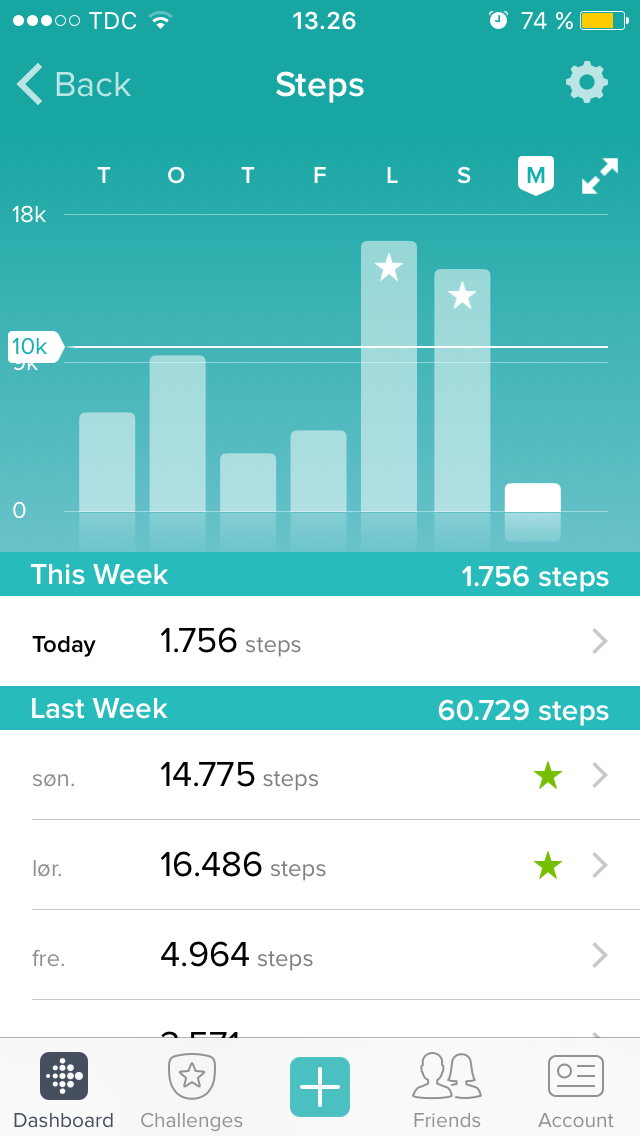
\includegraphics[width=0.45\textwidth]{figures/brugerfladesteps}
		\flushleft
		\caption{Oversigt over skridt taget for forhenværende dage, som graf (øverst) og tabel (nederst).}
	\end{minipage}
	\hfill
	\begin{minipage}[t]{0.45\textwidth}
		\label{fig:specifiksteps}
		\centering
		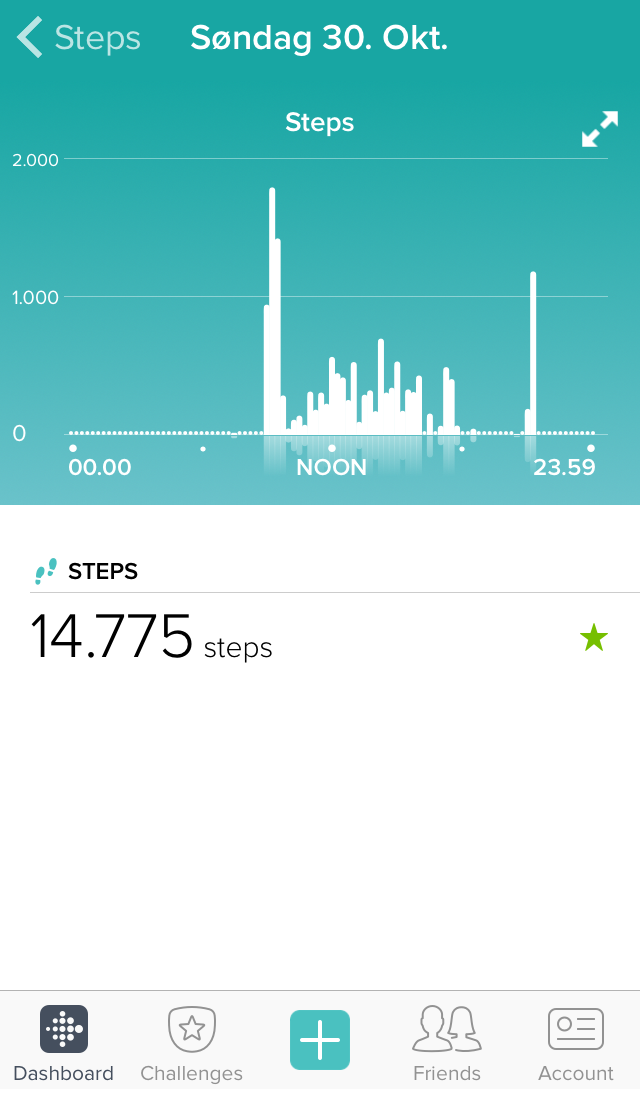
\includegraphics[width=0.45\textwidth]{figures/specifiksteps}
		\flushleft
		\vspace{12pt}
		\caption{Til venstre ses den grafiske oversigt over antal skridt taget, og højre figur viser skridt taget i en tabel.}
	\end{minipage}
\end{figure}

\noindent
Af \autoref{fig:brugerfladesteps} ses der øverst en graf over antal skridt taget inden for den sidste uge. Af grafen ses en hvid tværgående linje, der repræsenterer målet for antal skridt for dagen. Hertil ses at dage, hvor målet er blevet opfyldt, markeres med en stjerne.

Under grafen ses en oversigt over antal skridt taget for de forhenværende dage, rækkende tilbage til den første anvendelsesdato. Heraf ses ligeledes at dagene, hvor målet nåes, er indikeret med en stjerne. 

Ved at trykke på den givne dag eller en af de forhenværende dage, kan der ses en mere detaljeret oversigt over antal skridt taget i løbet af den pågældende dag. Dette ses af \autoref{fig:specifiksteps}, hvor det er muligt at se på hvilke tider af dagen, brugeren er mest aktiv.  


\subsection{Brugertilpasning} \label{sec:brugertilpasning}
Der er forskellige muligheder for at tilpasse armbåndet optimalt til den givne bruger. Heriblandt er der mulighed for at udskifte armbåndet til andre længder, og at tilpasse skridtlængden til den enkelte bruger. Foruden dette tilegner armbåndet sig til at blive brugt under forskellige vejrforhold, da Fitbit Flex er vandafvisende. 

\subsubsection{Forskellige Fitbit Flex armbånd}
Brugeren har mulighed for at vælge armbånd i to forskellige længder. Dette tillader muligheden for bedre tilpasning omkring håndleddet. Armbåndene kan ligeledes fås i forskellige farver.

\subsubsection{Kalibrering}
Applikationen vurderer som standard brugerens skridtlængde ud fra de angivne oplysninger ved oprettelsen af brugerkontoen. Brugeren har dog mulighed for at kalibrere denne værdi i tilfælde af, at brugeren opdager uoverensstemmelse mellem registrerede værdier og reelle værdier. Brugeren kan under indstillinger i applikationen ændre den pre-definerede skridtlængde til en mere passende værdi. Fitbit oplyser på deres support-hjemmeside guidelines for, hvordan brugeren selv udregner værdier til en mere passende skridtlængde.   

\begin{comment}
Hvad består teknologien af?
Hvor udbredt er teknologien?
Hvordan tilpasses teknologien den enkelte person?
Levetid for teknologien?
Hvilke muligheder er der for lagring og videregivelse af information til en læge?
\end{comment}
